\documentclass{standalone}

\usepackage[english]{babel}
\usepackage[linesnumbered, ruled, vlined]{algorithm2e}

\usepackage{caption}

% to create listings

\usepackage{listings, lstautogobble}
\lstset{
  autogobble=true,
  frame=single,
}

\lstdefinelanguage{coq}[Objective]{Caml}{
  morekeywords={Structure, Definition, Inductive, list, return},
  sensitive=true
}

% to define font size

\usepackage{ulem}
\usepackage{moresize}
\usepackage{anyfontsize}

% to use tikz and its libraries

\usepackage{tikz-timing}
\usepackage{tikz}

\usetikzlibrary{backgrounds}
\usetikzlibrary{positioning, calc, arrows, shapes, automata, petri, patterns}

% to use tikzmark, to place and refer to marks outside the current figure

\tikzset{every picture/.style={remember picture}}

% styles for transitions

\tikzset{transition/.append style={fill=black!20, thick}}
\tikzset{transition/.append style={fill=black!20, thick}}

% styles for test and inhib arcs.

\tikzstyle{test}=[pre, *-]
\tikzstyle{inhib}=[pre, o-]

% to use colors

\usepackage{xcolor}

%%%%%%%%%%%%%%%%%%%%%%%%%%%%%%%%%%%%%%%%%%%%%%%%%%
%                  BEGIN DOCUMENT                %
%%%%%%%%%%%%%%%%%%%%%%%%%%%%%%%%%%%%%%%%%%%%%%%%%%

\begin{document}

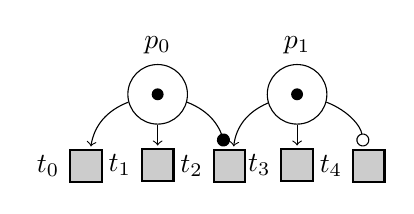
\begin{tikzpicture}

  \node[place, tokens=1] (p0) [label={above:$p_0$}] {};
  \node[transition] (t0) [below left=6mm of p0, label={left:$t_0$}] {}
  edge[pre, bend left] (p0);
  \node[transition] (t1) [below right=6mm of p0, label={left:$t_2$}] {}
  edge[test, bend right] (p0);

  \node[transition] (t3) [below=3mm of p0, label={left:$t_1$}] {}
  edge[pre] (p0);
  
  \node[place, tokens=1] (p1) [right=1cm of p0, label={above:$p_1$}] {};
  \node[transition] (t2) [below right=6mm of p1, label={left:$t_4$}] {}
  edge[inhib, bend right] (p1);
  \draw (t1) edge[pre, bend left] (p1);

  \node[transition] (t4) [below=3mm of p1, label={left:$t_3$}] {}
  edge[pre] (p1);
  
\end{tikzpicture}

\end{document}
%%% Local Variables:
%%% mode: latex
%%% TeX-master: t
%%% End:
